\begin{frame}
  \frametitle{Sparse Grids -- Examples}
  \topline
  \vspace{-10px}
  \begin{block}{Checkerboard dataset: non-linearity}
    \begin{figure}[!htp]

      \setbeamertemplate{caption}{\raggedright\insertcaption\par}
      \setbeamerfont{caption}{size=\footnotesize}
      \centering
      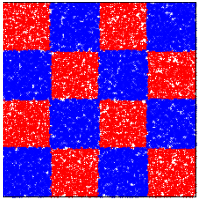
\includegraphics[width=0.4\textwidth]{images/example_checker1}
      \hspace{10px}
      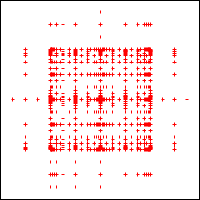
\includegraphics[width=0.4\textwidth]{images/example_checker2}
      \vspace{-8px}
      \caption{Checkerboard dataset and sparse grid
      (293 grid points) after 40 refinements}
    \end{figure}
    \begin{flushright}
      \tiny{\emph{(Dirk Pflüger -- Spatially Adaptive Sparse Grids for
          High-Dimensional Problems)}}
    \end{flushright}
  \end{block}
\end{frame}

\begin{frame}
  \frametitle{Sparse Grids -- Examples}
  \topline
  \vspace{-10px}
  \begin{block}{Checkerboard dataset: non-linearity}
    \begin{figure}[!htp]

      \setbeamertemplate{caption}{\raggedright\insertcaption\par}
      \setbeamerfont{caption}{size=\footnotesize}
      \centering
      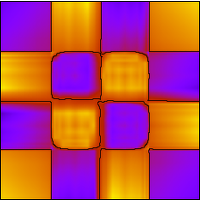
\includegraphics[width=0.4\textwidth]{images/example_checker3}
      \hspace{10px}
      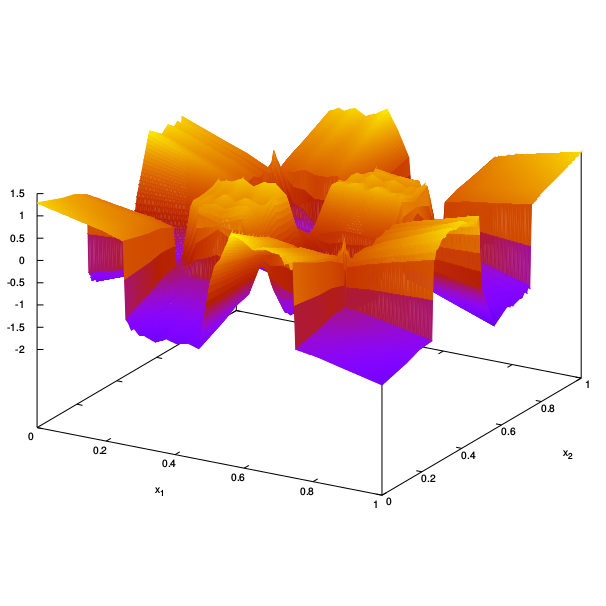
\includegraphics[width=0.4\textwidth]{images/example_checker4}
      \vspace{-8px}
      \caption{Decision manifold}
    \end{figure}
    \begin{flushright}
      \tiny{\emph{(Dirk Pflüger -- Spatially Adaptive Sparse Grids for
          High-Dimensional Problems)}}
    \end{flushright}
  \end{block}
\end{frame}


\begin{frame}
  \frametitle{Sparse Grids -- Examples}
  \topline
  \vspace{-10px}
  \begin{block}{Ripely dataset: noise and overfitting}
    \begin{figure}[!htp]
      \hspace{10px}
      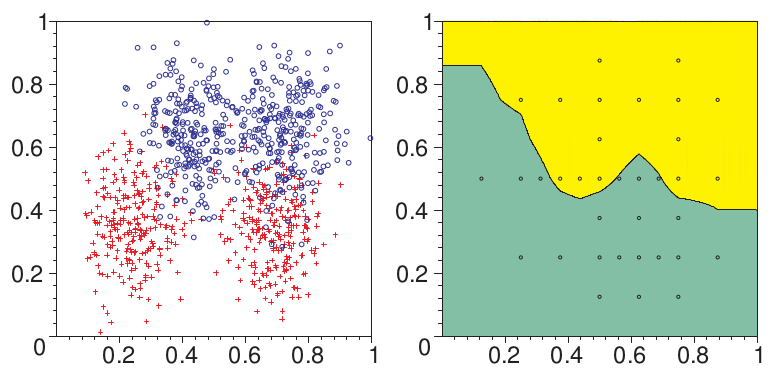
\includegraphics[width=0.8\textwidth]{images/example_ripely}
      \setbeamertemplate{caption}{\raggedright\insertcaption\par}
      \setbeamerfont{caption}{size=\footnotesize}
      \centering
      \vspace{-2px}
      \caption{Ripely dataset and sparse grid (34 grid points) after 8
      refinements}
    \end{figure}
    \begin{flushright}
      \tiny{\emph{(Dirk Pflüger -- Spatially Adaptive Sparse Grids for
          High-Dimensional Problems)}}
    \end{flushright}
  \end{block}
\end{frame}

%%% Local Variables:
%%% TeX-master: "slides"
%%% End:
